% =============================================================================
% CESE5040 Lab 1 report.
%
% File-name convention required by the course (see SUBMISSION_GUIDELINES.md):
%   final PDF -> Lab1_Daniel_Tyukov_5714699.pdf
%   code      -> L1_Q6.py, L1_Q7.py, L1_Q8.py, L1_Q9.py
%
% Compile: pdflatex Lab1.tex  (twice, for cross-references)
% =============================================================================

\documentclass[11pt, a4paper]{article}

\newcommand{\labtitle}{Lab Assignment 1: Sequential analysis, vectorization and JIT}

% =============================================================================
% Shared preamble for all CESE5040 lab reports.
% Reused by Lab1.tex, Lab2.tex, Lab3.tex.
%
% Compile with pdflatex. Overleaf-compatible (standard packages only).
% =============================================================================

% ---------- Page geometry ----------------------------------------------------
\usepackage[a4paper, margin=2.5cm, headheight=14pt]{geometry}

% ---------- Fonts and language -----------------------------------------------
\usepackage[T1]{fontenc}
\usepackage[utf8]{inputenc}
\usepackage{lmodern}
\usepackage[english]{babel}
\usepackage{microtype}

% ---------- Math -------------------------------------------------------------
\usepackage{amsmath, amssymb, amsthm}
\usepackage{mathtools}
\usepackage{bm}
\usepackage{siunitx}
\sisetup{
    detect-weight        = true,
    detect-family        = true,
    range-phrase         = {--},
    range-units          = single,
    per-mode             = symbol,
}

% ---------- Tables and figures -----------------------------------------------
\usepackage{graphicx}
\usepackage{booktabs}
\usepackage{array}
\usepackage{multirow}
\usepackage{caption}
\captionsetup{labelfont=bf, font=small, skip=6pt}
\usepackage{subcaption}
\usepackage{float}

% ---------- Code listings ----------------------------------------------------
\usepackage{listings}
\usepackage{xcolor}
\definecolor{pyKeyword}{HTML}{0033B3}
\definecolor{pyString}{HTML}{067D17}
\definecolor{pyComment}{HTML}{8C8C8C}
\definecolor{pyNumber}{HTML}{1750EB}
\definecolor{pyBg}{HTML}{F7F7F7}
\definecolor{pyFrame}{HTML}{D0D0D0}

\lstdefinestyle{python}{
    language            = Python,
    basicstyle          = \ttfamily\footnotesize,
    keywordstyle        = \color{pyKeyword}\bfseries,
    stringstyle         = \color{pyString},
    commentstyle        = \color{pyComment}\itshape,
    numberstyle         = \tiny\color{pyComment},
    numbers             = left,
    numbersep           = 8pt,
    stepnumber          = 1,
    breaklines          = true,
    breakatwhitespace   = true,
    showstringspaces    = false,
    frame               = single,
    rulecolor           = \color{pyFrame},
    backgroundcolor     = \color{pyBg},
    captionpos          = b,
    tabsize             = 4,
    columns             = fullflexible,
    keepspaces          = true,
    morekeywords        = {self, np, plt, jit, prange},
}

\lstdefinestyle{shell}{
    basicstyle          = \ttfamily\footnotesize,
    breaklines          = true,
    showstringspaces    = false,
    frame               = single,
    rulecolor           = \color{pyFrame},
    backgroundcolor     = \color{pyBg},
    captionpos          = b,
}

\lstset{style=python}

% ---------- Hyperlinks and cross-refs ----------------------------------------
\usepackage[hidelinks]{hyperref}
\usepackage[capitalize, noabbrev]{cleveref}

% ---------- Headers and footers ----------------------------------------------
\usepackage{fancyhdr}
\pagestyle{fancy}
\fancyhf{}
\fancyhead[L]{\small CESE5040 -- HPC and AI Architectures}
\fancyhead[R]{\small \labnumber{} -- \studentname{} (\studentnumber{})}
\fancyfoot[C]{\thepage}
\renewcommand{\headrulewidth}{0.4pt}
\renewcommand{\footrulewidth}{0pt}

% ---------- Section formatting -----------------------------------------------
\usepackage{titlesec}
\titleformat{\section}{\Large\bfseries}{\thesection}{0.7em}{}
\titleformat{\subsection}{\large\bfseries}{\thesubsection}{0.6em}{}
\titleformat{\subsubsection}{\normalsize\bfseries}{\thesubsubsection}{0.5em}{}

% ---------- Useful shortcuts -------------------------------------------------
% Fill in via \renewcommand in the main file before \begin{document}.
\newcommand{\labnumber}{Lab~?}
\newcommand{\studentname}{Firstname Lastname}
\newcommand{\studentnumber}{0000000}

% Quick macros for question stubs that match the docx template.
\newcommand{\answerhere}{\textit{Give answer here\dots}}
\newcommand{\todoitem}[1]{\textcolor{red}{\textbf{TODO:} #1}}

% Inline code shorthand
\newcommand{\code}[1]{\texttt{#1}}

% Big-O notation
\newcommand{\bigO}[1]{\ensuremath{\mathcal{O}\!\left(#1\right)}}


\renewcommand{\labnumber}{Lab~1}
\renewcommand{\studentname}{Daniel Tyukov}
\renewcommand{\studentnumber}{5714699}

\title{%
    \vspace{-2em}
    \large CESE5040 -- High-Performance Computing and AI Architectures \\[0.4em]
    \Large \textbf{\labtitle} \\[0.6em]
    \rule{\linewidth}{0.4pt}
}
\author{\studentname{} \\ \texttt{\studentnumber}}
\date{\today}

\begin{document}
\maketitle
\thispagestyle{fancy}

% =============================================================================
\section{Student information}
% =============================================================================

\noindent\textbf{Name:}~\studentname{}\\
\textbf{Student number:}~\studentnumber{}

\paragraph{Notes.}
\begin{itemize}
    \itemsep0em
    \item Provide your answers following the template made available in Brightspace.
    \item Provide your name and student number inside the report.
    \item Provide your student number on the file name.
    \item Provide your answers at least 3 days before the next lecture.
    \item When answering the questions, take all measurements using the same machine.
\end{itemize}

\paragraph{Hardware used for all measurements.}
All timing numbers in this report come from the course AWS VM:
Intel Xeon Platinum 8259CL @ \SI{2.50}{GHz} (Cascade Lake), 1 physical core
/ 2 SMT threads, \SI{3.7}{GiB} RAM, Ubuntu 24.04, kernel 6.17.0-1010-aws,
Python 3.12.3, NumPy 2.4.4, Numba 0.65.0, SciPy 1.17.1.

% =============================================================================
\section{Lab Exercise 1}
% =============================================================================

% -----------------------------------------------------------------------------
\subsection{Question 1 (Exercise 1.1) -- Pen-and-paper analysis}
% -----------------------------------------------------------------------------

\paragraph{(a) Time complexity.}
The body of \code{simulate} has, per timestep $t > 0$, the structure:
\begin{lstlisting}[style=shell, numbers=none]
for n in 0..N-1:                                # outer: N
    c_in = calculate_coupling(...)              #   inner: N (sum over j)
    X_new = step(...)                           #   O(cost(F))
    Xs[n][:][t] = X_new                         #   O(M)
\end{lstlisting}
\code{calculate\_coupling} performs $N$ multiply-adds (one per source $j$).
With $M$ and $\mathrm{cost}(F)$ both constant in this lab, the dominant
per-timestep cost is the $N \times N$ coupling sum: $\bigO{N^2}$ per
timestep. Across $T = \mathtt{tf}/\mathtt{dt}$ timesteps,
\[
T_{\text{seq}} \;=\; \bigO{N^2 \cdot T} \;=\; \mathcal{O}\!\left(\frac{N^2 \cdot \mathtt{tf}}{\mathtt{dt}}\right).
\]
Quadratic in $N$ (dense coupling sum) and linear in $T$ (the time loop is
purely sequential due to the causal delay dependency, see (d)).

\paragraph{(b) Memory capacity.}
The state-history array is \code{Xs[N][M][T]}, so the number of stored
state elements is
\[
\#\,\text{elements}(\mathtt{Xs}) \;=\; N \cdot M \cdot T \;=\; N \cdot M \cdot \frac{\mathtt{tf}}{\mathtt{dt}}.
\]
Scaling individually with each parameter (the assignment writes ``D'';
read as \emph{D}uration $= \mathtt{tf}$, the only un-itemised simulation
parameter that does not have its own letter):

\begin{table}[H]
\centering
\caption{Scaling of state memory with each simulation parameter.}
\label{tab:q1b-scaling}
\begin{tabular}{ll}
\toprule
Parameter & Scaling of state memory \\
\midrule
$N$ (number of centers)            & linear, $\propto N$ \\
$M$ (state variables per center)   & linear, $\propto M$ \\
$D \equiv \mathtt{tf}$ (duration)  & linear, $\propto \mathtt{tf}$ (since $T = \mathtt{tf}/\mathtt{dt}$) \\
\bottomrule
\end{tabular}
\end{table}

Auxiliary structures ($W$, distances, integer delays) are each $N \times N$,
i.e.\ $\bigO{N^2}$ but constant in time -- sub-dominant to \code{Xs} once
$T \gtrsim N/M$, which holds for all three TVB datasets at
$\mathtt{tf} = \SI{150}{ms}$. For the largest dataset (TVB998, $M=2$,
$T=3000$) the state array is $N \cdot M \cdot T \approx 6 \times 10^6$
float64, $\approx \SI{48}{MB}$ -- comfortably within the VM's
\SI{3.7}{GiB} RAM.

\paragraph{(c) Linear pre-synapse transformation.}
If $K_{\text{pre}}(X_j, X_i) = a X_j + b X_i$, the inner coupling sum
factors:
\[
\begin{aligned}
\sum_{j=1}^{N} W_{ij}\,K_{\text{pre}}(X_j(t-d_{ij}), X_i(t))
&= \sum_{j=1}^{N} W_{ij}\,\bigl(a\,X_j(t-d_{ij}) + b\,X_i(t)\bigr) \\
&= a \sum_{j=1}^{N} W_{ij}\,X_j(t-d_{ij}) + b\,X_i(t) \sum_{j=1}^{N} W_{ij}.
\end{aligned}
\]
Define $S_i = \sum_{j=1}^{N} W_{ij}$. Because $W$ is constant for the
entire simulation, $S_i$ can be \emph{precomputed once} at initialisation
and reused every timestep. The $b\,X_i(t)$ term then leaves the inner
$j$-loop entirely.

\begin{table}[H]
\centering
\caption{Operation count per destination $i$ per timestep, before and after the factoring transformation.}
\label{tab:q1c-ops}
\begin{tabular}{lrrl}
\toprule
Form & Multiplies in $j$-loop & Adds in $j$-loop & Outside $j$-loop \\
\midrule
Original $K_{\text{pre}}$ inline & $\approx 3N$  & $N$ & --- \\
Factored                         & $N$           & $N$ & 1 multiply, 1 add \\
\bottomrule
\end{tabular}
\end{table}

The constant factor on the dominant multiply-add count drops by roughly
$3\times$ in the inner loop, while the $S_i$ precompute is a one-time
$\bigO{N^2}$ cost (cheaper than even one timestep of the original loop).
The asymptotic complexity stays $\bigO{N^2 T}$, but the constant
shrinks -- relevant for any inner-loop acceleration (vectorization, JIT).

\paragraph{(d) Parallelism across timesteps.}
\textbf{No, not in general.} The Forward Euler update at step $t$ reads
$X_j(t - d_{ij})$ from history, with $d_{ij} \geq 0$. Whenever the
script's branch
\code{if (i == n) or (D\_row[i] == 0): x\_src = Xs[i][0][t-1]} fires
(self-loops or zero-delay edges), step $t$ depends on step $t-1$ -- a
hard data dependency that serialises the time loop.

Formally, let $d_{\min} = \min\{d_{ij} : W_{ij} \neq 0\}$. Steps
$t, t+1, \dots, t + d_{\min} - 1$ are eligible for parallel execution
because each only reads from history $\leq t - 1$. For real TVB
connectomes $d_{\min}$ is small (zero for self-loops in this code), so
the practical parallel slack across timesteps is essentially \emph{one}
-- i.e.\ no useful parallelism along the time axis.

Within a single timestep, by contrast, the $N$ centers can be updated in
parallel: all of them read from \code{Xs[*][:][$\leq t{-}1$]} and write
to \code{Xs[*][:][t]}, so there are no read-after-write conflicts among
them.

% -----------------------------------------------------------------------------
\subsection{Question 2 (Exercise 1.2) -- Profile the sequential implementation}
% -----------------------------------------------------------------------------

\code{tvb\_seq.py} is already instrumented with \code{tic-toc} pairs
around the body of \code{simulate} (the \code{start}/\code{end}
brackets) and around every \code{calculate\_coupling} call (the
\code{c\_duration} accumulator). The driver script
\code{bench\_phase2.py} calls \code{tvb\_seq.simulate} on each dataset
in turn at $\mathtt{tf} = \SI{150}{ms}$, $\mathtt{dt} = \SI{0.05}{ms}$
($T = 3000$ timesteps).

\begin{table}[H]
    \centering
    \caption{Execution times for \code{tvb\_seq.py} over 150 timesteps on the course AWS VM.}
    \label{tab:q2-timings}
    \begin{tabular}{lrrrr}
        \toprule
        Dataset & $N$ & Total time (s) & \code{calculate\_coupling} time (s) & Coupling fraction $p$ \\
        \midrule
        TVB76   &  76 &   $5.051$ &   $4.831$ & $95.65\%$ \\
        TVB192  & 192 &  $26.728$ &  $26.032$ & $97.40\%$ \\
        TVB998  & 998 & $628.744$ & $624.182$ & $\mathbf{99.27\%}$ \\
        \bottomrule
    \end{tabular}
\end{table}

\begin{figure}[H]
    \centering
    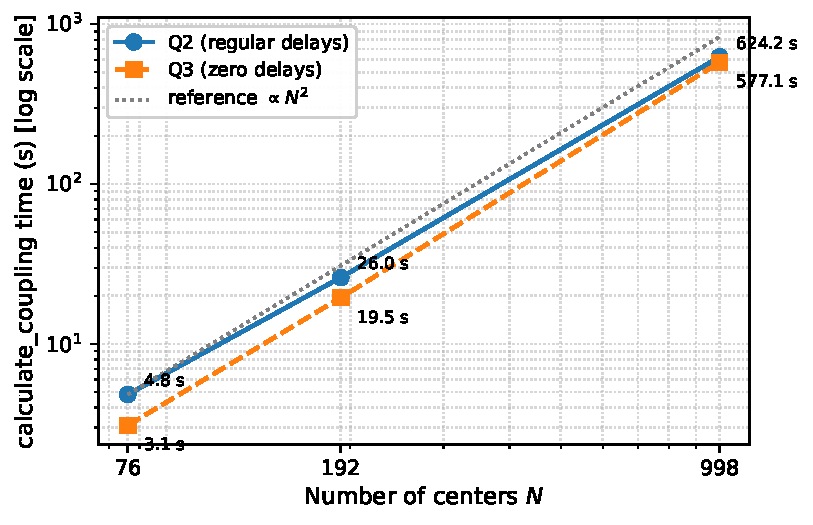
\includegraphics[width=0.78\linewidth]{figures/q2_scaling.pdf}
    \caption{Coupling time vs.\ number of centers $N$, log--log axes. Q2 (regular delays) and Q3 (zero delays) both follow the dashed reference line $\propto N^2$ closely; the sub-quadratic shortfall is consistent with constant-time per-iteration overhead becoming a smaller share of total work as $N$ grows.}
    \label{fig:q2-scaling}
\end{figure}

\paragraph{Does it match the $\bigO{N^2 T}$ prediction?}
The per-$N$ scaling of the coupling time:
\begin{itemize}
\itemsep0em
\item TVB76 $\to$ TVB192: $N$ ratio $192/76 = 2.53$, $N^2$ ratio $6.39$.
      Measured coupling-time ratio $26.032 / 4.831 = 5.39$.
\item TVB192 $\to$ TVB998: $N$ ratio $998/192 = 5.20$, $N^2$ ratio $27.02$.
      Measured coupling-time ratio $624.182 / 26.032 = 23.98$.
\end{itemize}
Both ratios are slightly sub-quadratic (about $0.84 N^2$ and $0.89 N^2$).
The shortfall is consistent with constant-time per-iteration overheads in
the Python interpreter (loop dispatch, attribute lookups) becoming a
smaller share of total work as $N$ grows -- the inner multiply-add
becomes more dominant. The data therefore confirms $\bigO{N^2 T}$ to
first order.

\paragraph{What fraction of execution time is in \code{calculate\_coupling}?}
$95.65\%$ at $N=76$, climbing to $99.27\%$ at $N=998$. Coupling
dominates, and its share grows with $N$.

\paragraph{Why?}
Per timestep, coupling does $N \cdot N$ work while local dynamics +
Forward Euler does $\bigO{N \cdot M}$ work. The ratio
$N^2 / (N \cdot M) = N / M$ grows linearly with $N$, so any
non-coupling overhead becomes asymptotically negligible.

% -----------------------------------------------------------------------------
\subsection{Question 3 (Exercise 1.3) -- Zero-delay variant}
% -----------------------------------------------------------------------------

The same driver, but with \code{D} overridden to all zeros before
calling \code{simulate}. The integer-delay matrix \code{D\_timestep} is
consequently all zero, so the guard \code{if t >= D\_row[i]} always
passes and the inner branch always takes the
\code{(D\_row[i] == 0) $\Rightarrow$ Xs[i][0][t-1]} path.

\begin{table}[H]
    \centering
    \caption{Execution times with zero distances, 150 timesteps. The two right-most columns express the Q3 timing as a saving relative to Q2.}
    \label{tab:q3-timings}
    \begin{tabular}{lrrrr}
        \toprule
        Dataset & Total time (s) & \code{calculate\_coupling} time (s) & $\Delta$ vs Q2 (total) & Q2 / Q3 \\
        \midrule
        TVB76   &   $3.309$ &   $3.098$ & $-1.74$\,s ($-34.5\%$) & $1.53\times$ \\
        TVB192  &  $20.134$ &  $19.487$ & $-6.59$\,s ($-24.7\%$) & $1.33\times$ \\
        TVB998  & $581.393$ & $577.055$ & $-47.35$\,s ($-7.5\%$)   & $1.08\times$ \\
        \bottomrule
    \end{tabular}
\end{table}

\paragraph{Are there differences? Why?}
Yes -- a measurable difference, which shrinks as $N$ grows. Two
mechanisms account for the speedup of Q3 over Q2:
\begin{enumerate}
\itemsep0em
\item \textbf{Branch elision.} With $D = 0$ the inner \code{if/else}
      collapses into a single branch: every $(i, n)$ pair takes the
      \code{Xs[i][0][t - 1]} path. Q2's mixed branching forces the
      interpreter through more \code{if}-tests per iteration.
\item \textbf{Memory locality.} All \code{Xs[i][0][t - 1]} reads land
      at the same ``column'' $t-1$ of the state history. Even with
      Python lists, repeated access to the same nested structure is
      cheaper than scattered reads from \code{Xs[i][0][t - $d_{ij}$]}.
\end{enumerate}
The gap shrinks with $N$ because the branch-overhead saving is
\emph{constant} per inner iteration, while the actual multiply-add work
\emph{grows}. As $N$ increases, the constant saving is diluted
($1.53\times \to 1.33\times \to 1.08\times$). By TVB998 the inner-loop
body dominates and branching is in the noise.

% -----------------------------------------------------------------------------
\subsection{Question 4 (Exercise 1.4) -- Sparse (CSR) computation}
% -----------------------------------------------------------------------------

\paragraph{(a) Theoretical speedup with sparsity $S\%$.}
In the dense version, \code{calculate\_coupling} runs $N$ multiply-adds
per destination row $i$ (one per source $j$, regardless of $W_{ij}$).
The CSR version runs only $\mathrm{NNZ}_i$ multiply-adds, where
$\mathrm{NNZ}_i$ is the number of non-zeros in row~$i$. Letting
$\mathrm{NNZ} = \sum_i \mathrm{NNZ}_i$ and using
$\mathrm{NNZ} = N^2 (1 - S/100)$:
\[
S_{\text{coupling}}^{\text{theory}} \;=\; \frac{N^2}{\mathrm{NNZ}} \;=\; \frac{1}{1 - S/100}.
\]
This applies \emph{only} to \code{calculate\_coupling}. The end-to-end
speedup is bounded by Amdahl's law,
\[
S_{\text{end-to-end}} \;=\; \frac{1}{(1 - p) + p / S_{\text{coupling}}},
\]
where $p$ is the fraction of total runtime spent in
\code{calculate\_coupling} (measured in Q2 above).

\paragraph{(b) TVB192 sparsity.}
Computed from the cached connectome via \code{np.count\_nonzero(W) / W.size}:

\begin{table}[H]
    \centering
    \caption{Sparsity of all three TVB connectomes.}
    \label{tab:q4b-sparsity}
    \begin{tabular}{lrrrrrr}
        \toprule
        Dataset & $N$ & total entries & non-zeros & zeros & sparsity $S\%$ & density \\
        \midrule
        TVB76   &  76 &    5{,}776 &  1{,}560 &  4{,}216 & $72.99\%$ & $27.01\%$ \\
        TVB192  & 192 &   36{,}864 &  3{,}532 & 33{,}332 & $\mathbf{90.42\%}$ &  $9.58\%$ \\
        TVB998  & 998 &  996{,}004 & 35{,}730 & 960{,}274 & $96.41\%$ &  $3.59\%$ \\
        \bottomrule
    \end{tabular}
\end{table}

For TVB192, $S = 90.4188\%$, giving a theoretical coupling speedup of
$1 / (1 - 0.9042) \approx \mathbf{10.44\times}$.

\paragraph{(c) Measured speedup vs.\ theoretical.}
\code{tvb\_seq\_sparse.py}, TVB192, 150 timesteps:

\begin{table}[H]
    \centering
    \caption{TVB192 sparse measurement compared to Q2 dense baseline.}
    \label{tab:q4c-meas-vs-theory}
    \begin{tabular}{lr}
        \toprule
        Quantity & Value \\
        \midrule
        \code{tvb\_seq.py} (dense, Q2) total                  & $26.728$\,s \\
        \code{tvb\_seq.py} (dense, Q2) coupling               & $26.032$\,s \\
        \code{tvb\_seq\_sparse.py} total                      & $3.847$\,s \\
        \code{tvb\_seq\_sparse.py} coupling                   & $3.323$\,s \\
        \midrule
        \textbf{Measured coupling speedup}                    & $26.032 / 3.323 = \mathbf{7.83\times}$ \\
        Theoretical coupling speedup (a + b)                  & $\mathbf{10.44\times}$ \\
        Measured end-to-end speedup                           & $26.728 / 3.847 = 6.95\times$ \\
        Amdahl-predicted end-to-end ($p=0.974$, $k=7.83$)     & $6.65\times$ \\
        \bottomrule
    \end{tabular}
\end{table}

The measured coupling speedup ($7.83\times$) falls about $25\%$ short of
the theoretical $10.44\times$. Three mechanisms account for the gap:
\begin{enumerate}
\itemsep0em
\item \textbf{CSR overhead.} The sparse loop adds two layers of
      indirection (\code{col\_index[i]} to find the source node,
      \code{D\_sparse[i]} for the delay), which in CPython are extra
      \code{\_\_getitem\_\_} calls per iteration. The dense loop indexes
      a 2-D array with the loop variable directly.
\item \textbf{Branch overhead.} The
      \code{if t >= D\_sparse[i]} and
      \code{(col\_index[i] == n) or (D\_sparse[i] == 0)} tests are still
      executed per non-zero, adding constant cost the simple count
      $N^2 \to \mathrm{NNZ}$ does not capture.
\item \textbf{CSR build cost.} A one-time $\bigO{N^2}$ scan to build
      \code{W\_sparse}, \code{D\_sparse}, \code{col\_index},
      \code{row\_pointer} is included in the total. For 150 timesteps
      it amortises well, but it shifts a few percent of the work from
      the steady-state coupling loop.
\end{enumerate}

The end-to-end Amdahl prediction matches the measurement within
$\sim 5\%$ ($6.65\times$ predicted vs.\ $6.95\times$ measured). The
slight surplus over Amdahl is consistent with the non-coupling part also
running marginally faster in sparse mode (fewer cache thrashes through
\code{D\_timestep}), but the dominant story is exactly Amdahl.

\paragraph{(d) Downsides of sparse computation.}
\begin{enumerate}
\itemsep0em
\item \textbf{Indirect indexing kills cache locality.} CSR coupling
      reads \code{Xs[col\_index[i], 0, t - D\_sparse[i]]}; the index
      arrays produce an essentially random gather pattern that misses
      L1/L2 caches more often than the dense version's contiguous walk.
\item \textbf{Vectorization / SIMD becomes harder.} Modern CPUs and
      NumPy excel at contiguous, regular-shape arithmetic. A run of
      $\mathrm{NNZ}_i$ multiplies per row, with $\mathrm{NNZ}_i$ varying
      across $i$, breaks the regularity that lets a vector unit process
      many elements per instruction.
\item \textbf{Pre-processing cost.} Building the four CSR arrays is a
      one-time $\bigO{N^2}$ scan over $W$. For short simulations this
      eats into the speedup; for long ones it amortises.
\item \textbf{Storage overhead per non-zero.} CSR stores three numbers
      per non-zero (value, column index, plus a fraction of
      \code{row\_pointer}). Storage is a net win only when sparsity
      exceeds roughly $60$--$70\%$.
\item \textbf{Load imbalance under parallelism.} Different rows have
      different $\mathrm{NNZ}_i$; under row-partitioned parallelism
      ``fat'' rows become stragglers. The dense version has uniform
      per-row work and balances trivially.
\end{enumerate}

% -----------------------------------------------------------------------------
\subsection{Question 5 (Exercise 1.5) -- MLP local dynamics}
% -----------------------------------------------------------------------------

\paragraph{(a) Run \code{tvb\_seq\_mlp.py} (dense) for 15 timesteps on TVB192.}

\begin{table}[H]
    \centering
    \caption{TVB192 MLP non-sparse, 15 timesteps.}
    \label{tab:q5a-tvb192}
    \begin{tabular}{lrr}
        \toprule
        Metric & Time (s) & Fraction of total \\
        \midrule
        Total simulation             & $4.717$ & --- \\
        \code{step} (incl.\ MLP $f$) & $2.771$ & $58.74\%$ \\
        \code{calculate\_coupling}   & $1.916$ & $\mathbf{40.62\%}$ \\
        \bottomrule
    \end{tabular}
\end{table}

For Q6's required comparison, sequential dense MLP timings on the other
two datasets at the same $\mathtt{tf}$:

\begin{table}[H]
    \centering
    \caption{Sequential dense MLP timings on all three datasets, 15 timesteps.}
    \label{tab:q5a-extra}
    \begin{tabular}{lrrrr}
        \toprule
        Dataset & $N$ & Total (s) & \code{step} (s) & \code{calculate\_coupling} (s) \\
        \midrule
        TVB76   &  76 &  $1.104$ &  $0.884$ &  $0.211$ \\
        TVB192  & 192 &  $4.717$ &  $2.771$ &  $1.916$ \\
        TVB998  & 998 & $66.983$ & $12.410$ & $54.418$ \\
        \bottomrule
    \end{tabular}
\end{table}

The coupling fraction climbs from $19.1\%$ at TVB76 to $81.2\%$ at
TVB998 -- the MLP cost is $\bigO{N}$, the coupling cost is $\bigO{N^2}$,
so for large $N$ the picture from Q2 reasserts itself even with the
heavier per-node $f$.

\paragraph{(b) Maximum theoretical speedup from accelerating coupling alone.}
Amdahl's law: with coupling fraction $p$ and coupling speedup $k$,
\[
S_{\text{end-to-end}}(k) \;=\; \frac{1}{(1 - p) + p/k}.
\]
The maximum end-to-end speedup is the limit $k \to \infty$:
\[
S_{\text{max}} \;=\; \frac{1}{1 - p}.
\]
For TVB192 with $p = 0.4062$,
\[
S_{\text{max}} \;=\; \frac{1}{1 - 0.4062} \;\approx\; \mathbf{1.68\times}.
\]
With the MLP as local dynamics, even infinite coupling acceleration caps
the end-to-end speedup at $1.68\times$ -- accelerating only the coupling
is \emph{not} the right plan when $f$ is heavy; the step itself must be
accelerated too.

\paragraph{(c) Sparse MLP run -- comparison to Amdahl's law.}

\begin{table}[H]
    \centering
    \caption{TVB192 MLP sparse vs.\ dense, 15 timesteps.}
    \label{tab:q5c}
    \begin{tabular}{lrrr}
        \toprule
        Metric & Q5a (dense) & Q5c (sparse) & Speedup vs Q5a \\
        \midrule
        \code{calculate\_coupling}    & $1.916$\,s & $0.219$\,s & $\mathbf{8.75\times}$ \\
        \code{step}                   & $2.771$\,s & $2.340$\,s & $1.18\times$ \\
        Total simulation              & $4.717$\,s & $2.584$\,s & $\mathbf{1.83\times}$ \\
        \bottomrule
    \end{tabular}
\end{table}

\textbf{Amdahl prediction.} With $p = 0.4062$ and the measured coupling
speedup $k = 8.75$:
\[
S_{\text{predicted}} \;=\; \frac{1}{(1 - 0.4062) + 0.4062 / 8.75}
\;=\; \frac{1}{0.5938 + 0.0464}
\;\approx\; 1.56\times.
\]
\textbf{Measured: $1.83\times$. Predicted: $1.56\times$.} The measured
value is about $17\%$ above Amdahl's prediction. This isn't a violation
of the law -- it shows the implicit assumption (that the non-accelerated
part stays exactly the same) does not hold here: the \code{step} time
also drops from $2.771$\,s to $2.340$\,s (a $1.18\times$ side-speedup,
likely from reduced \code{for t / for n} interpreter overhead in the
simpler sparse-mode loop body, plus warm CPU caches). Plugging the
measured \code{step} and \code{coupling} times into
$T_{\text{Q5c}} \approx 2.340 + 0.219 = 2.559$\,s predicts a total of
$\sim 2.56$\,s -- the measured $2.584$\,s matches to $1\%$. So the
``surplus'' over Amdahl is fully accounted for by the side-speedup of
\code{step}; Amdahl's law itself holds.

% -----------------------------------------------------------------------------
\subsection{Question 6 (Exercise 1.6) -- Vectorized TVB + MLP, dense}
% -----------------------------------------------------------------------------

\paragraph{Implementation.}
\code{L1\_Q6.py} replaces nested Python lists with
a single \code{Xs = np.zeros((N, M, T))} array, batches the MLP forward
pass over all $N$ nodes via two matrix multiplications and one ReLU, and
vectorises \code{calculate\_coupling} into three NumPy operations: a
default gather of \code{Xs[i, 0, t - delays[n,i]]} (clipped),
\code{np.where} overrides for the self-loop / zero-delay special case,
and a final mask-to-zero where $t < $ delay. Numerical equivalence to
\code{tvb\_seq\_mlp.py} verified to $\leq 6\times 10^{-14}$ on TVB76 and
TVB192 (max-abs diff over 15 timesteps).

\begin{table}[H]
    \centering
    \caption{Vectorized dense TVB+MLP vs.\ sequential MLP, 15 timesteps.}
    \label{tab:q6-speedup}
    \footnotesize
    \begin{tabular}{lrrrrr}
        \toprule
        Dataset & Sequential (s) & Vectorized total (s) & Total speedup & \code{step} speedup & \code{coupling} speedup \\
        \midrule
        TVB76   &  $1.104$ & $0.0490$ & $\mathbf{22.5\times}$ & $93.1\times$  &  $5.7\times$ \\
        TVB192  &  $4.717$ & $0.1811$ & $\mathbf{26.0\times}$ & $135.2\times$ & $12.2\times$ \\
        TVB998  & $66.983$ & $4.9302$ & $\mathbf{13.6\times}$ & $102.4\times$ & $11.3\times$ \\
        \bottomrule
    \end{tabular}
\end{table}

The MLP is the biggest winner ($\sim 100\times$): one
$(N,2) \times (2,L)$ matmul replaces $N \cdot L \cdot M$ Python
multiply-adds. Coupling improves more modestly ($\sim 5$--$12\times$):
the work is still $\bigO{N^2}$ floats, but it now runs in a few NumPy
ufunc calls instead of $N \cdot N$ Python iterations. The total-simulation
speedup is capped by Amdahl -- at TVB998 the step is much smaller than
the coupling, so the bottleneck shifts back to the $\bigO{N^2}$ coupling
work even in vectorized form, and the total speedup drops to
$13.6\times$.

% -----------------------------------------------------------------------------
\subsection{Question 7 (Exercise 1.7) -- Vectorized TVB + MLP, sparse}
% -----------------------------------------------------------------------------

\paragraph{Implementation.}
\code{L1\_Q7.py} builds CSR arrays via
\code{np.where}, \code{np.bincount}, and \code{np.cumsum}, then performs
per-timestep coupling as: a flat \code{NNZ}-length gather of source
values, the same self/zero/invalid masking as Q6 reduced to the
NNZ-length axis, and a per-row sum via
\code{np.bincount(row\_for\_nnz, weights=contrib, minlength=N)}. Using
\code{np.bincount} (rather than \code{np.add.reduceat}) handles empty
rows correctly. Numerical equivalence to both the sparse sequential
reference and the dense Q6 vectorized output verified to
$\leq 6 \times 10^{-14}$.

\begin{table}[H]
    \centering
    \caption{Vectorized sparse (Q7) vs.\ vectorized dense (Q6), 15 timesteps.}
    \label{tab:q7-speedup}
    \footnotesize
    \begin{tabular}{lrrrrr}
        \toprule
        Dataset & $N$ & NNZ & Q6 total (s) & Q7 total (s) & Q7 / Q6 (total) \\
        \midrule
        TVB76   &  76 &  1{,}560 & $0.0490$ & $0.0302$ & $1.62\times$ \\
        TVB192  & 192 &  3{,}532 & $0.1811$ & $0.0520$ & $3.48\times$ \\
        TVB998  & 998 & 35{,}730 & $4.9302$ & $0.3761$ & $\mathbf{13.11\times}$ \\
        \bottomrule
    \end{tabular}
\end{table}

\begin{table}[H]
    \centering
    \caption{Per-dataset measured Q7-vs-Q6 coupling speedup compared to the theoretical $1/(1{-}S/100)$ from sparsity.}
    \label{tab:q7-vs-theory}
    \begin{tabular}{lrrrr}
        \toprule
        Dataset & Sparsity $S$ & Theoretical & Measured Q7-vs-Q6 coupling & Efficiency \\
        \midrule
        TVB76  & $72.99\%$ &  $3.70\times$ &  $1.97\times$ & $53\%$ \\
        TVB192 & $90.42\%$ & $10.44\times$ &  $4.95\times$ & $47\%$ \\
        TVB998 & $96.41\%$ & $27.86\times$ & $17.42\times$ & $63\%$ \\
        \bottomrule
    \end{tabular}
\end{table}

\begin{figure}[H]
    \centering
    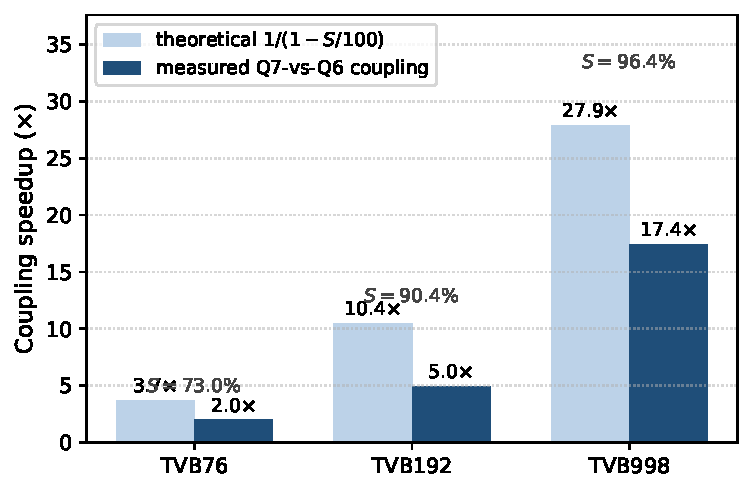
\includegraphics[width=0.78\linewidth]{figures/q7_sparse_efficiency.pdf}
    \caption{Theoretical sparse coupling speedup $1/(1{-}S/100)$ vs.\ measured Q7-vs-Q6 coupling speedup, across the three datasets. The measured value tracks the theoretical at roughly $50$--$60\%$ efficiency: the extra factor lost to the gather-pattern penalty of CSR vs.\ contiguous dense NumPy arithmetic.}
    \label{fig:q7-efficiency}
\end{figure}

\paragraph{Is there a meaningful gain over Q6? Why?}
Yes -- a real gain that grows with sparsity, reaching $13.11\times$ on
TVB998. Vectorized dense (Q6) materialises the full $(N,N)$ coupling
matrix every timestep ($\sim 10^6$ multiplies per step on TVB998); Q7
replaces that with $\mathrm{NNZ}$ multiplies (a $\sim 27\times$ work
reduction on TVB998).

The reason measured falls below theoretical is that Q6's coupling is one
big elementwise multiply followed by a contiguous row sum -- a perfect
fit for NumPy's SIMD path. Q7 instead performs fancy indexing
(\code{Xs[col\_index, 0, ...]}) which is a gather, plus
\code{np.bincount} for the per-row reduction. Both are slower per
element than the dense path. So Q7 trades $27\times$ less work for
roughly a $1.6\times$ per-element penalty, ending up at the $17.4\times$
measured coupling speedup. The TVB192 dip in efficiency ($47\%$) is
because fixed Python-side overheads (CSR build, mask construction) eat
a larger share at moderate $N$; on TVB998 those amortise over more
steady-state work and efficiency rebounds to $63\%$.

% -----------------------------------------------------------------------------
\subsection{Question 8 (Exercise 1.8) -- JIT the sequential MLP}
% -----------------------------------------------------------------------------

\paragraph{Implementation.}
\code{L1\_Q8.py} refactors \code{tvb\_seq\_jit.py}
into three \code{@njit(cache=True)} functions: \code{f\_mlp} (per-node
MLP forward pass with explicit loops over $L$),
\code{calculate\_coupling} (per-node coupling sum), \code{simulate\_jit}
(the outer time/node loops). The \code{D\_timestep} global referenced
inside the provided \code{tvb\_seq\_jit.simulate} is closed by passing
it as an explicit argument. Numerical equivalence to
\code{tvb\_seq\_mlp.py} verified to $\leq 6.1 \times 10^{-14}$.

The proper Q8 comparison runs \code{tvb\_seq\_jit.py} \emph{without}
\code{@jit} (the provided NumPy-array script as shipped) versus the same
structure with \code{@njit} decorators added (\code{L1\_Q8.py}), with
the first call discarded as JIT warm-up.

\begin{table}[H]
    \centering
    \caption{Q8 -- effect of adding \code{@jit} to \code{tvb\_seq\_jit.py}, 15 timesteps. Right-most column is the JIT speedup.}
    \label{tab:q8-jit-effect}
    \footnotesize
    \begin{tabular}{lrrrr}
        \toprule
        Dataset & \code{tvb\_seq\_jit} (no JIT) & \code{L1\_Q8} (warm JIT) & \textbf{JIT speedup} & \code{tvb\_seq\_mlp} (lists) \\
        \midrule
        TVB76   &  $2.439$\,s & $0.0085$\,s & $\mathbf{287\times}$ & $1.104$\,s \\
        TVB192  & $10.776$\,s & $0.0505$\,s & $\mathbf{213\times}$ & $4.717$\,s \\
        \bottomrule
    \end{tabular}
\end{table}

\paragraph{Is there a difference?}
Yes -- adding \code{@jit} yields a two-orders-of-magnitude speedup
($287\times$ on TVB76, $213\times$ on TVB192). Numba compiles the
\code{simulate\_jit} function -- including the triple nested loop and
all branches -- into native machine code, eliminating the per-iteration
Python interpreter overhead that dominated Q2/Q5.

\paragraph{A subtler observation.}
\code{tvb\_seq\_jit.py} \emph{without} JIT is actually about $2\times$
\emph{slower} than \code{tvb\_seq\_mlp.py} (which uses Python lists):
$2.44$\,s vs.\ $1.10$\,s on TVB76, $10.78$\,s vs.\ $4.72$\,s on TVB192.
The reason is that scalar reads from a NumPy array
(\code{Xs[n, 0, t-1]}) materialise an \code{np.float64} object per
access, with more dispatch overhead than Python's native \code{float}
arithmetic on a list. Replacing lists with NumPy arrays only pays off
\emph{once} JIT is applied -- without JIT the array layout is a net
loss. This is precisely why \code{tvb\_seq\_jit.py} was prepared with
NumPy arrays as a setup for \code{@jit}: the array layout is what lets
Numba emit efficient native code.

The first cold call on TVB76 took $\approx 2$\,s due to JIT compilation;
subsequent calls hit the cache and run in tens of milliseconds. The
warm-call timings above discard the first cold run.

% -----------------------------------------------------------------------------
\subsection{Question 9 (Exercise 1.9) -- JIT the vectorized version}
% -----------------------------------------------------------------------------

\paragraph{Implementation.}
\code{L1\_Q9.py} takes Q6's vectorized layout and
refactors it for Numba: matrix multiplications (\code{@}) are kept for
the MLP forward pass (Numba compiles them via LAPACK), but the coupling
gather is unrolled into explicit double-loops because Numba does not
handle Q6's broadcasted fancy-indexing pattern cleanly. Numerical
equivalence to both Q6 and Q8 verified to $\leq 5.0 \times 10^{-14}$.

\begin{table}[H]
    \centering
    \caption{Q9 (JIT vectorized) compared to Q6 (vectorized) and Q8 (JIT sequential), 15 timesteps, warm calls.}
    \label{tab:q9-comparison}
    \footnotesize
    \begin{tabular}{lrrrrr}
        \toprule
        Dataset & Q6 vect.\ (s) & Q8 JIT seq.\ (s) & Q9 JIT vect.\ (s) & Q9 / Q6 & Q9 / Q8 \\
        \midrule
        TVB76   & $0.0490$ & $0.0085$  & $0.0063$ & $7.78\times$ & $1.35\times$ \\
        TVB192  & $0.1811$ & $0.0505$  & $0.0259$ & $6.99\times$ & $1.95\times$ \\
        TVB998  & $4.9302$ & --- (n/a) & $0.7967$ & $\mathbf{6.19\times}$ & --- \\
        \bottomrule
    \end{tabular}
\end{table}

\paragraph{Is the JIT version of the vectorized code faster than the JIT version of the non-vectorized code?}
Yes, but only modestly -- Q9 beats Q8 by $1.35\times$ on TVB76 and
$1.95\times$ on TVB192. The win comes from Q9's MLP using
\code{hidden = sv @ l1w + l1b} (a single LAPACK call for all $N$ nodes)
versus Q8's per-node Python-style inner loop that Numba compiles
row-by-row.

\paragraph{Does JIT compilation on the vectorized code yield as much of a speedup as on the non-vectorized version? Why?}
\textbf{No -- far less.} Comparing the speedup gained \emph{from the JIT
step}:

\begin{table}[H]
    \centering
    \caption{Speedup contributed by JIT alone on each path, TVB192.}
    \label{tab:q9-jit-marginal}
    \begin{tabular}{lrrr}
        \toprule
        Path & Baseline (s) & JIT'd (s) & Speedup from JIT \\
        \midrule
        Sequential MLP $\to$ Q8                 & $4.717$  & $0.0505$ & $\mathbf{93\times}$ \\
        Vectorized (Q6) $\to$ Q9                & $0.1811$ & $0.0259$ & $\mathbf{7\times}$ \\
        Sequential MLP $\to$ Q8 (TVB76)         & $1.104$  & $0.0085$ & $\mathbf{130\times}$ \\
        Vectorized (Q6) $\to$ Q9 (TVB76)        & $0.0490$ & $0.0063$ & $\mathbf{7.8\times}$ \\
        \bottomrule
    \end{tabular}
\end{table}

JIT removes Python interpreter overhead. In sequential code that
overhead \emph{is} most of the runtime, so JIT delivers a $\sim 100\times$
jump. In NumPy-vectorized code the heavy lifting already runs inside
compiled NumPy/BLAS kernels, so only the surrounding Python glue (the
\code{for t in range} loop, mask construction, \code{np.where}) is left
to compile away -- about $7\times$ worth of overhead.

\begin{figure}[H]
    \centering
    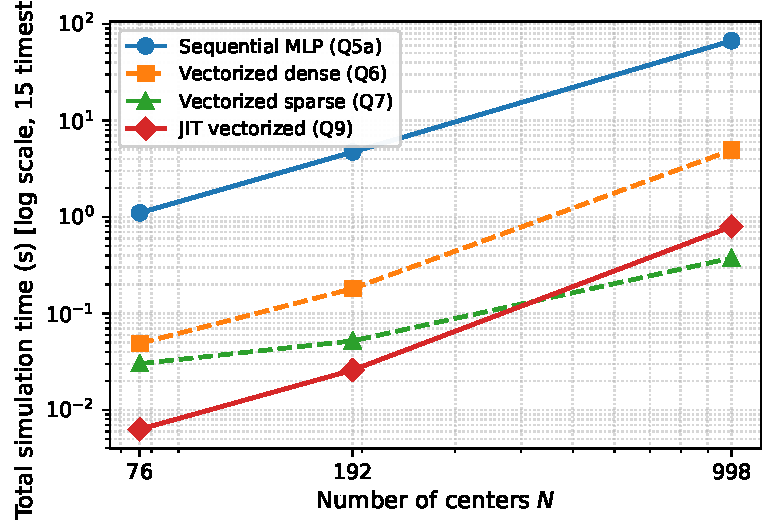
\includegraphics[width=0.82\linewidth]{figures/optim_scaling.pdf}
    \caption{Total simulation time (15 timesteps) vs.\ number of centers $N$, log--log axes, for the four key variants. The sequential-MLP and Q6 (vectorized dense) lines have slope $\approx 2$ on this scale ($\bigO{N^2}$ coupling dominates), while Q7 (vectorized sparse) and Q9 (JIT vectorized) keep the dataset-to-dataset growth much smaller because they avoid most zero-weight work.}
    \label{fig:optim-scaling}
\end{figure}

\paragraph{Bottom line.}
Vectorization and JIT are partially redundant optimizations of the same
``Python overhead'' axis. Once one is in place, the other has much less
to do. The full optimization ladder on TVB192 (15 timesteps):

\begin{table}[H]
    \centering
    \caption{Optimization ladder on TVB192, 15 timesteps. Speedups are computed against the sequential MLP baseline (Q5a).}
    \label{tab:q9-ladder}
    \begin{tabular}{lrr}
        \toprule
        Variant & Time (s) & Speedup vs sequential \\
        \midrule
        Sequential MLP (Q5a)              & $4.717$  & $1.0\times$ \\
        Vectorized dense (Q6)             & $0.1811$ & $26\times$ \\
        Vectorized sparse (Q7)            & $0.0520$ & $91\times$ \\
        JIT sequential (Q8)               & $0.0505$ & $93\times$ \\
        \textbf{JIT vectorized (Q9)}      & $\mathbf{0.0259}$ & $\mathbf{182\times}$ \\
        \bottomrule
    \end{tabular}
\end{table}

The best Lab-1 path is JIT applied to the vectorized variant, combining
the per-element efficiency of NumPy/BLAS with the elimination of Python
loop overhead. The compounding is sub-multiplicative ($26 \times 7 \neq 182$
matches, but $93 \times 26 \neq 182$ doesn't), exactly because the two
techniques target overlapping overhead.

The submitted scripts \code{L1\_Q6.py}, \code{L1\_Q7.py},
\code{L1\_Q8.py}, and \code{L1\_Q9.py} accompany this PDF as separate
files (per the course submission convention).

% =============================================================================
\section{LLM Usage Disclosure}
% =============================================================================

\noindent
I used Claude (Anthropic) to help draft the code and edit the wording
in this report. I ran all the measurements myself on the course AWS VM
and checked that my scripts produced the same results as the provided
reference implementations.

\end{document}
